% chapter1.tex
\chapter{Examples}

\section{Theorem System}

\defn{Definition Name}{ref1}{
    A definition.
}

\thm{Theorem Name}{ref1}{
    A theorem.
}

\thmp{Theorem Name with Proof}{ref2}{
    A theorem with a proof.
}{
    This is the proof of the theorem.
}

\lem{Lemma Name}{ref1}{
    A lemma.
}

\lemp{Lemma Name with Proof}{ref2}{
    A lemma with a proof.
}{
    This is the proof of the lemma.
}

\prop{Proposition Name}{ref1}{
    A proposition.
}{
    This is the proof of the proposition.
}

\cor{Corollary Name}{ref1}{
    A corollary.
}{
    This is the proof of the corollary.
}

\clm{Claim Name}{
    A claim.
}{
    This is the proof of the claim.
}

\ex{
    This is an example.
}

\exer{
    Exercise example.
}

\rmk{
    This is a remark.
}

\pf{
    Veniam velit incididunt deserunt est proident consectetur non velit ipsum voluptate nulla quis. Ea ullamco consequat non ad amet cupidatat cupidatat aliquip tempor sint ea nisi elit dolore dolore. 

    Laboris labore magna dolore eiusmod ea ex et eiusmod laboris. Et aliquip cupidatat reprehenderit id officia pariatur. 
}

\section{Pictures}

\begin{figure}[H]
    \center
    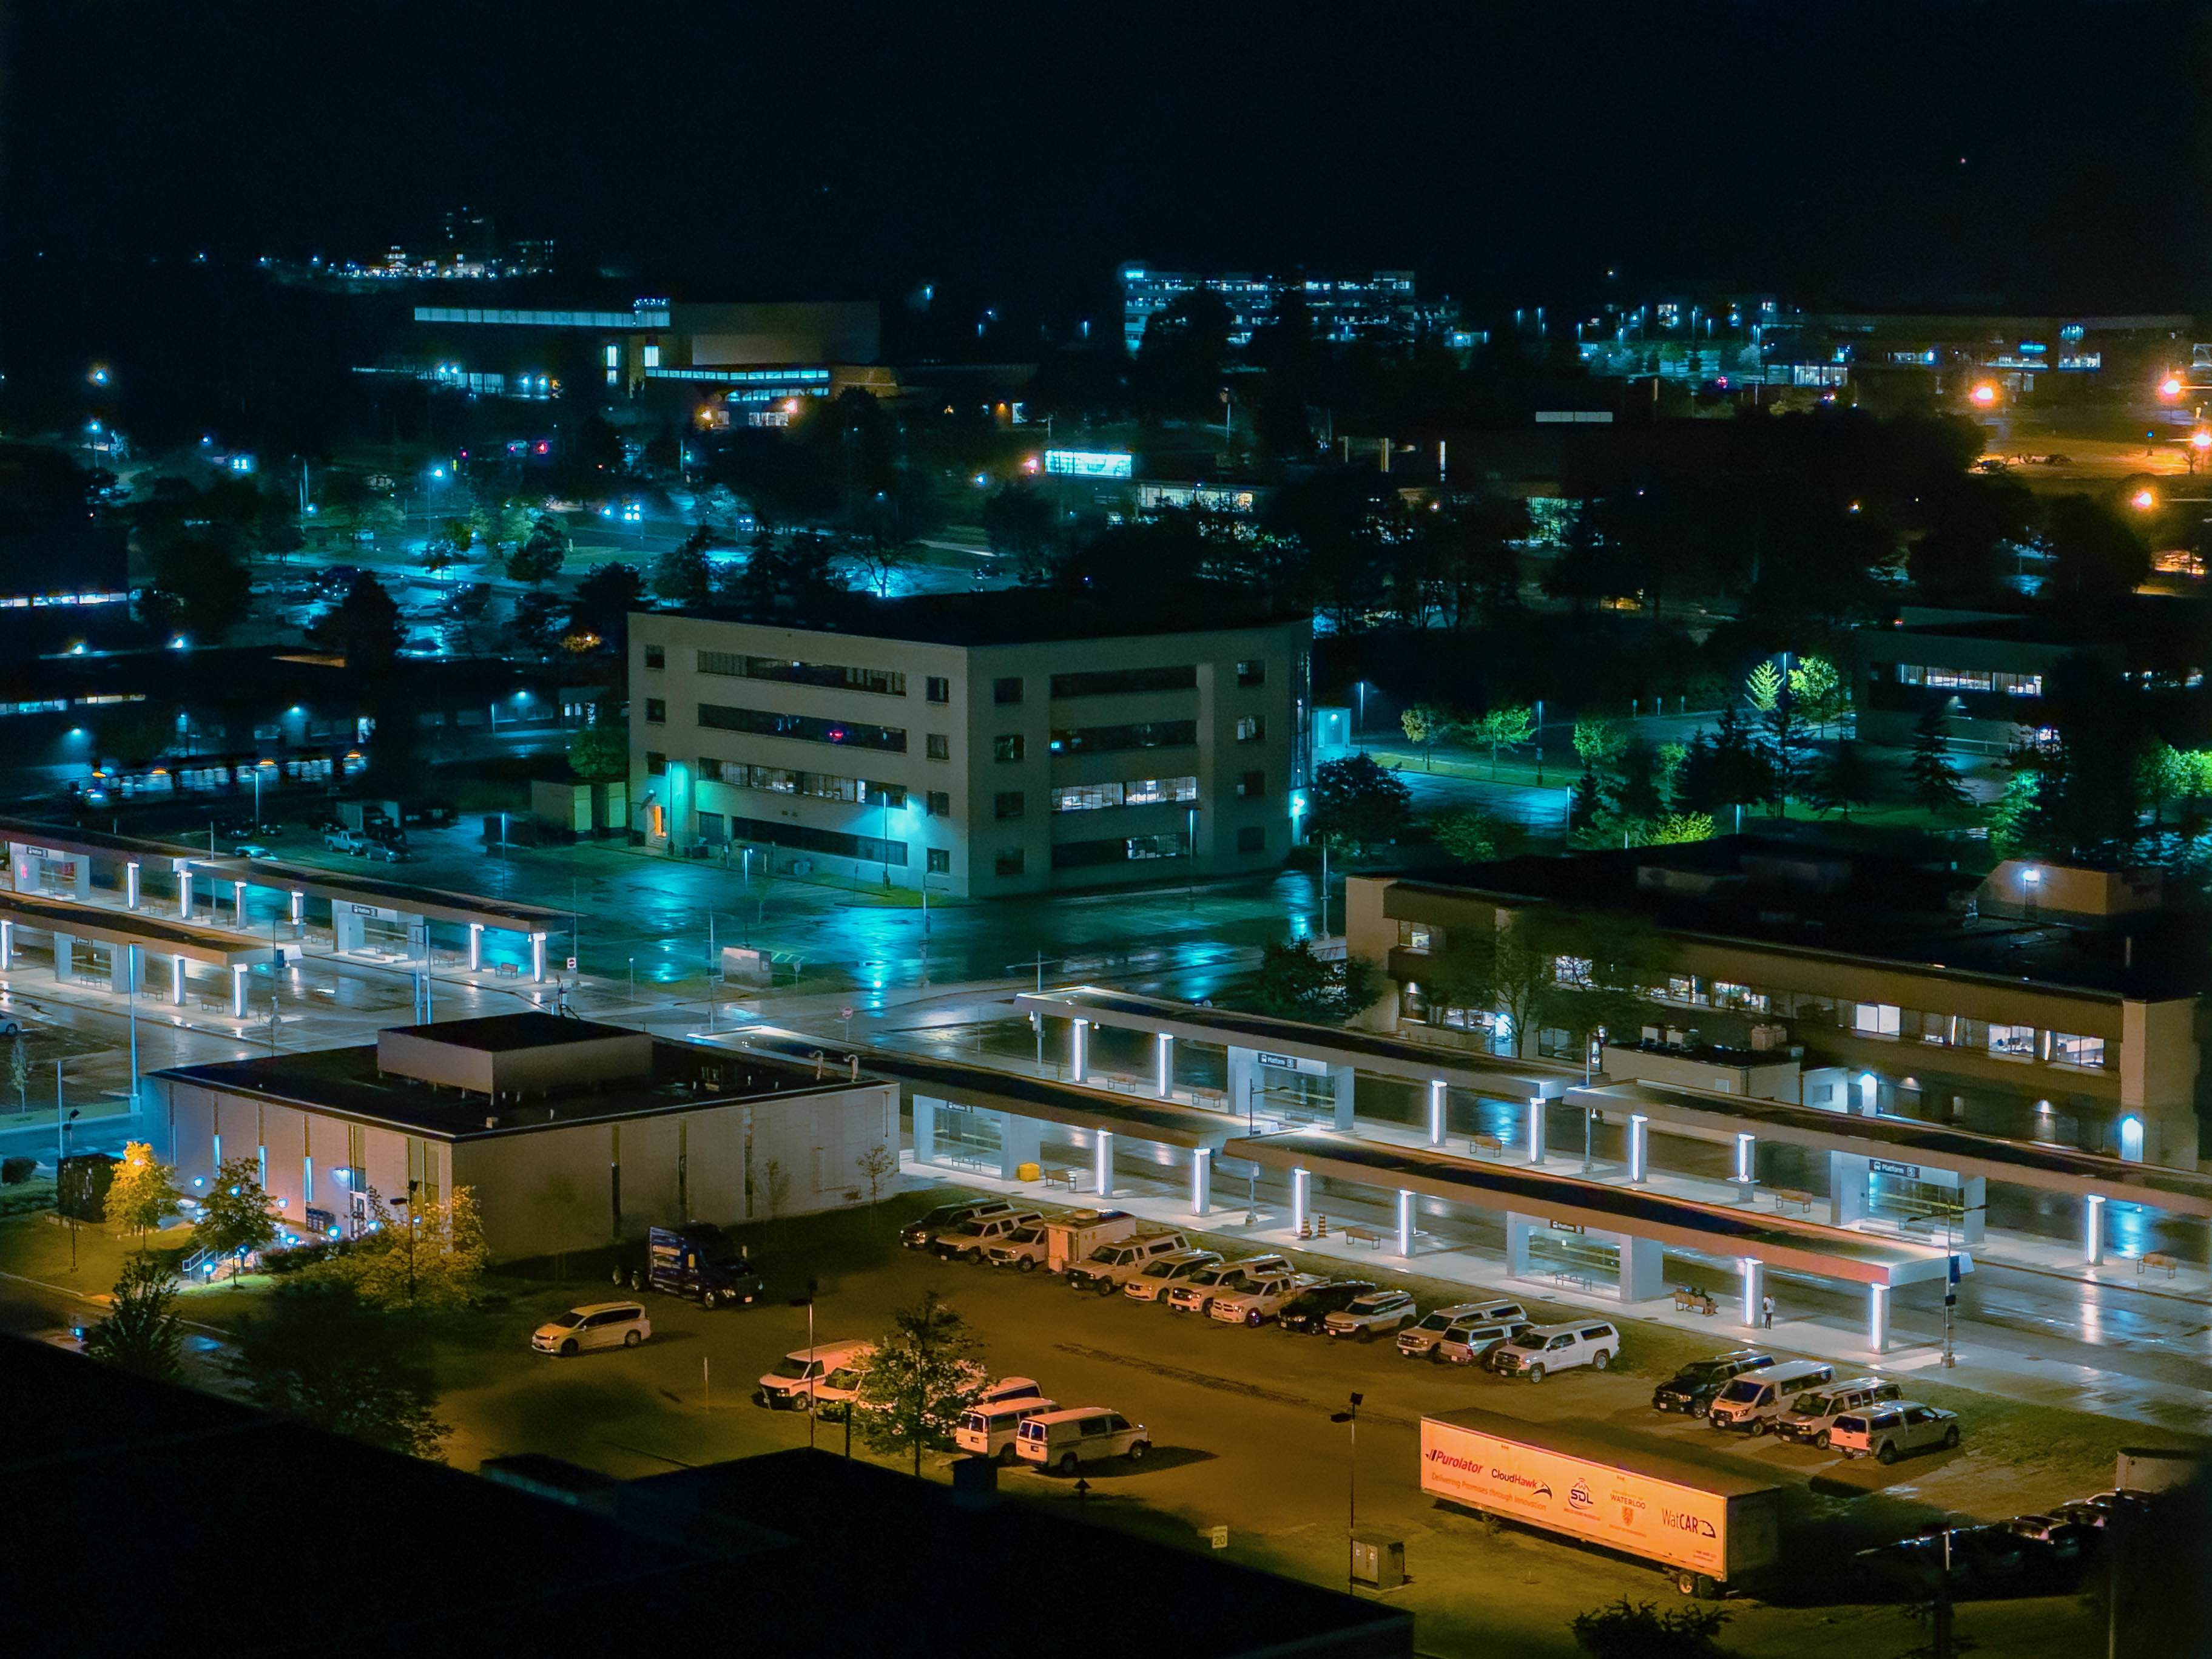
\includegraphics[scale=0.1]{src/img/loo.jpg}
    \caption{Waterloo, ON}
\end{figure}